% fig-mrt2-pipeline.tex
% CS2 (Magenta RealTime 2) per-frame streaming loop under the 40 ms deadline.
% data: surgical-inference.md Section 6.2 (per-frame pipeline order + SPSC ring +
%       AVAudioSourceNode + control-rate prompt chain) and Section 6.7 (shipped
%       placement: rolling temporal on GPU, in-graph depth rollout FP16 on CPU,
%       NCHW codec decoder on ANE; composed p50 ~29 ms/frame = temporal 12.2 +
%       depth 8.4 + decoder 8.3 on A17 Pro). Deadline 40 ms/frame (25 Hz), Section 6.1.
% Build: tectonic paper/figures/fig-mrt2-pipeline.tex
\documentclass[border=6pt]{standalone}
\usepackage[T1]{fontenc}
\usepackage[scaled]{helvet}
\renewcommand{\familydefault}{\sfdefault}
\usepackage{sansmath}
\usepackage{tikz}
\usetikzlibrary{arrows.meta,positioning,fit,backgrounds,calc,decorations.pathreplacing}

\definecolor{cmlgpu}{HTML}{CDE4F2}   % Core ML on CPU+GPU  (temporal, shipped)
\definecolor{cmlcpu}{HTML}{DED0EA}   % Core ML on CPU FP16 (depth rollout)
\definecolor{cmlane}{HTML}{C7E9C0}   % Core ML on CPU+ANE  (codec decoder, NCHW)
\definecolor{swiftc}{HTML}{FDE3C4}   % native host (Swift / Accelerate)
\definecolor{audblk}{HTML}{E8E8E8}   % audio I/O
\definecolor{edgec}{HTML}{444444}
\definecolor{deadl}{HTML}{B00020}    % deadline accent

\begin{document}
\sansmath
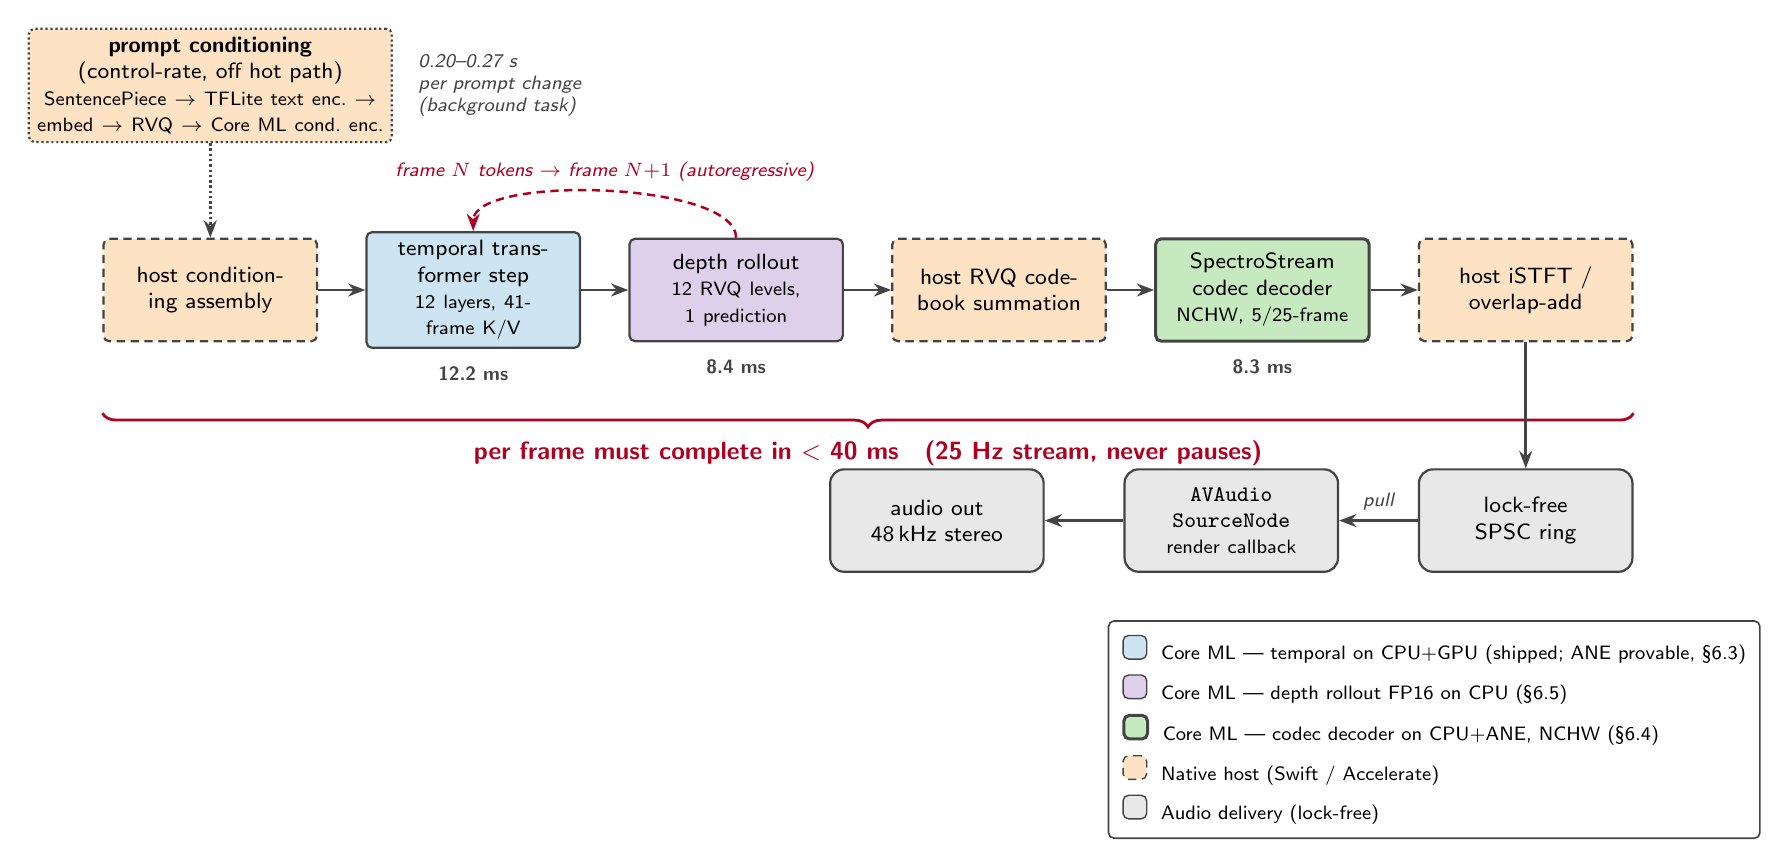
\begin{tikzpicture}[
  font=\sffamily\footnotesize,
  >={Stealth[length=2.2mm]},
  every node/.style={transform shape},
  box/.style={rectangle, rounded corners=2pt, draw=edgec, line width=0.8pt,
              align=center, inner sep=3pt, minimum height=13mm, text width=25mm},
  gpu/.style={box, fill=cmlgpu},
  cpu/.style={box, fill=cmlcpu},
  ane/.style={box, fill=cmlane, line width=1.1pt},
  host/.style={box, fill=swiftc, densely dashed},
  aud/.style={box, fill=audblk, rounded corners=5pt},
  ms/.style={font=\sffamily\scriptsize\bfseries, text=edgec},
  ann/.style={font=\sffamily\scriptsize\itshape, text=edgec, align=center},
  flow/.style={->, draw=edgec, line width=0.9pt},
]

% ---- per-frame generation row (left -> right) ----
\node[host] (cond) {host conditioning assembly};
\node[gpu, right=6mm of cond] (temp) {temporal transformer step\\{\scriptsize 12 layers, 41-frame K/V}};
\node[cpu, right=6mm of temp] (depth) {depth rollout\\{\scriptsize 12 RVQ levels, 1 prediction}};
\node[host, right=6mm of depth] (sum) {host RVQ codebook summation};
\node[ane, right=6mm of sum] (codec) {SpectroStream codec decoder\\{\scriptsize NCHW, 5/25-frame}};
\node[host, right=6mm of codec] (istft) {host iSTFT /\\overlap-add};

% ---- per-Core ML-stage frame cost (A17 Pro, Section 6.7) ----
\node[ms, below=1mm of temp.south]  {12.2 ms};
\node[ms, below=1mm of depth.south] {8.4 ms};
\node[ms, below=1mm of codec.south] {8.3 ms};

% ---- delivery row ----
\node[aud, below=16mm of istft] (ring) {lock-free\\SPSC ring};
\node[aud, left=10mm of ring] (source) {\texttt{AVAudio}\\\texttt{SourceNode}\\{\scriptsize render callback}};
\node[aud, left=10mm of source] (spk) {audio out\\48\,kHz stereo};

% ---- generation flow ----
\draw[flow] (cond) -- (temp);
\draw[flow] (temp) -- (depth);
\draw[flow] (depth) -- (sum);
\draw[flow] (sum) -- (codec);
\draw[flow] (codec) -- (istft);
\draw[flow] (istft.south) -- (ring.north);
\draw[flow] (ring) -- node[ann, above, yshift=0pt]{pull} (source);
\draw[flow] (source) -- (spk);

% ---- autoregressive loopback: frame N tokens -> frame N+1 temporal step ----
\draw[flow, deadl, densely dashed]
  (depth.north) to[out=90, in=90, looseness=0.55]
  node[ann, text=deadl, above, pos=0.5]{frame $N$ tokens $\to$ frame $N{+}1$ (autoregressive)}
  (temp.north);

% ---- 40 ms deadline brace over the generation path ----
\begin{scope}[on background layer]
  \draw[decorate, decoration={brace, amplitude=5pt, mirror}, draw=deadl, line width=1pt]
    ($(cond.south west)+(0,-9mm)$) -- ($(istft.south east)+(0,-9mm)$)
    node[midway, below=6pt, font=\sffamily\small\bfseries, text=deadl]
      {per frame must complete in $<$ 40 ms \; (25 Hz stream, never pauses)};
\end{scope}

% ---- control-rate prompt chain (off the hot path) ----
\node[host, above=12mm of cond, text width=44mm, minimum height=9mm,
      fill=swiftc, densely dotted] (prompt)
  {\textbf{prompt conditioning} (control-rate, off hot path)\\
   {\scriptsize SentencePiece $\to$ TFLite text enc.\ $\to$ embed $\to$ RVQ $\to$ Core ML cond.\ enc.}};
\node[ann, right=2mm of prompt.east, align=left] {0.20--0.27 s\\per prompt change\\(background task)};
\draw[flow, densely dotted] (prompt.south) -- (cond.north);

% ---- engine legend ----
\node[anchor=north west, draw=edgec, line width=0.6pt, rounded corners=2pt,
      inner sep=5pt, align=left, font=\sffamily\scriptsize] (leg)
      at ($(source.south west)+(-2mm,-6mm)$) {%
  {\tikz\node[draw=edgec,line width=0.5pt,fill=cmlgpu,minimum width=3mm,minimum height=3mm,inner sep=0pt]{};}~~Core ML --- temporal on CPU+GPU (shipped; ANE provable, \S6.3)\\[2.5pt]
  {\tikz\node[draw=edgec,line width=0.5pt,fill=cmlcpu,minimum width=3mm,minimum height=3mm,inner sep=0pt]{};}~~Core ML --- depth rollout FP16 on CPU (\S6.5)\\[2.5pt]
  {\tikz\node[draw=edgec,line width=1.1pt,fill=cmlane,minimum width=3mm,minimum height=3mm,inner sep=0pt]{};}~~Core ML --- codec decoder on CPU+ANE, NCHW (\S6.4)\\[2.5pt]
  {\tikz\node[draw=edgec,line width=0.5pt,densely dashed,fill=swiftc,minimum width=3mm,minimum height=3mm,inner sep=0pt]{};}~~Native host (Swift / Accelerate)\\[2.5pt]
  {\tikz\node[draw=edgec,line width=0.5pt,fill=audblk,minimum width=3mm,minimum height=3mm,inner sep=0pt]{};}~~Audio delivery (lock-free)};
\end{tikzpicture}
\end{document}
